\documentclass[letterpaper,10pt]{article}

\usepackage{tabularx} % extra features for tabular environment
\usepackage{amsmath}  % improve math presentation
\usepackage{graphicx} % takes care of graphic including machinery
\usepackage[margin=1in,letterpaper]{geometry} % decreases margins
\usepackage{cite} % takes care of citations
\usepackage[final]{hyperref} % adds hyper links inside the generated pdf file
\usepackage{ctex}
\usepackage{titlesec}
%\usepackage{CJKutf8, CJK}
\usepackage{makecell}                 % 三线表-竖线
\usepackage{booktabs}                 % 三线表-短细横线
% \usepackage{natbib}
\usepackage{graphicx}				  % 表格单元格逆时针
\usepackage{multirow}				  % 合并单元格
\usepackage{array}
\usepackage{amssymb}				  % 勾
\usepackage{amsmath}
\usepackage{longtable}                % 导入 longtable 宏包,表格自动换行
\usepackage{caption}
\usepackage{subcaption}               % 设置子图
\usepackage{color}					  % 文本颜色包
\usepackage{xcolor}
\usepackage{bbm}					  % 输入指示函数
\usepackage{tablefootnote}			  % 表格注释
\usepackage{pythonhighlight}

\usepackage{listings}                 % 导入代码块
\usepackage{xcolor}
\lstset{
	numbers=left, 
	tabsize=1,
	columns=flexible, 
	numberstyle=  \small, 
	keywordstyle= \color{ blue!70},
	commentstyle= \color{red!50!green!50!blue!50}, 
	frame=shadowbox, % 阴影效果
	rulesepcolor= \color{ red!20!green!20!blue!20} ,
	escapeinside=``, % 英文分号中可写入中文
	xleftmargin=2em,
	xrightmargin=2em, 
	aboveskip=1em,
} 

\hypersetup{
	colorlinks=true,       % false: boxed links; true: colored links
	linkcolor=blue,        % color of internal links
	citecolor=blue,        % color of links to bibliography
	filecolor=magenta,     % color of file links
	urlcolor=blue         
}
%++++++++++++++++++++++++++++++++++++++++
\titleformat{\section}{\Large\bfseries\songti}{\thesection}{1em}{}
\titleformat{\subsection}{\large\bfseries\songti}{\thesubsection}{1em}{}
\titleformat{\subsubsection}{\normalsize\bfseries\songti}{\thesubsubsection}{1em}{}
\titleformat{\paragraph}{\small\bfseries\songti}{\paragraph}{1em}{}
\titleformat{\subparagraph}{\footnotesize\bfseries\songti}{\subparagraph}{1em}{}

\begin{document}
	
	
	\title{\songti \zihao{4}6月23日-6月30日工作汇报}
	\author{\textrm{Ku Jui}}
	\date{\textrm{June 2023}}
	\maketitle
	
	\renewcommand{\figurename}{Figure} % 可以重新定义abstract,因为ctex会覆盖thebibliography
	% 	\begin{abstract}
		%		In this experiment we studied a very important physical effect by measuring the
		%		dependence of a quantity $V$ of the quantity $X$ for two different sample
		%		temperatures.  Our experimental measurements confirmed the quadratic dependence
		%		$V = kX^2$ predicted by Someone's first law. The value of the mystery parameter
		%		$k = 15.4\pm 0.5$~s was extracted from the fit. This value is
		%		not consistent with the theoretically predicted $k_{theory}=17.34$~s. We attribute %this
		%		discrepancy to low efficiency of our $V$-detector.
		%	\end{abstract}
	\renewcommand{\contentsname}{Contents}
	\renewcommand{\tablename}{Table}
	\tableofcontents  % 自动生成目录
	
	\section{Pre-Knowledge}
		
	\subsection{Transformer}
	
	在Attention引入以前,seq2seq模型处理机器翻译task最大的问题就是由于对于长距离的信息不能有效的提取和记忆,导致了信息的大量丢失。即使在引入Attention之后,也会因为对关系的捕捉不足,而出现翻译效果不理想。因为在这样的翻译任务中,需要发现的关系有三种:
	
	\begin{itemize}
		\item [(1)]
			源句内部的关系;
		\item [(2)]
			目标句内部的关系;
		\item [(3)]
			源句与目标句之间的关系;
	\end{itemize}
	
	之前的seq2seq模型只捕捉了源句与目标句之间的关系,而忽略了源句、目标句内部的关系,源句内部和目标句内部还是在用RNN,对远距离信息的捕捉能力很差。除了对远距离关系难以学习的不足以外,RNN 还有一点不足,那就是训练慢。因为它默认是按时序来进行处理的,一个个单词词从左到右看过去,导致 RNN 不能像 CNN 一样,充分利用 GPU 的并行运算优势。
	
	\subsubsection{Idea}
	
	\begin{itemize}
	
	\item [(1)] 刚刚提到了翻译任务存在有三种关系,原来的模型只学到其中一种,即源句与目标句之间的关系,Transformer\textbf{引入self-attention的机制将三种关系全部做了学习。}
	\item [(2)]	
	Transformer\textbf{提出了multi-head attention的机制},分别学习对应的三种关系,使用了全Attention的结构。
		
	\item[(2)] 
	对于词语的位置,Transformer \textbf{使用positional encoding机制进行数据预处理},增大了模型的并行性,取得了更好的实验效果。
	
	\end{itemize}
	
	\subsubsection{Architecture}
	
	\begin{figure}[htbp]
		% read manual to see what [ht] means and for other possible options
		\centering 
		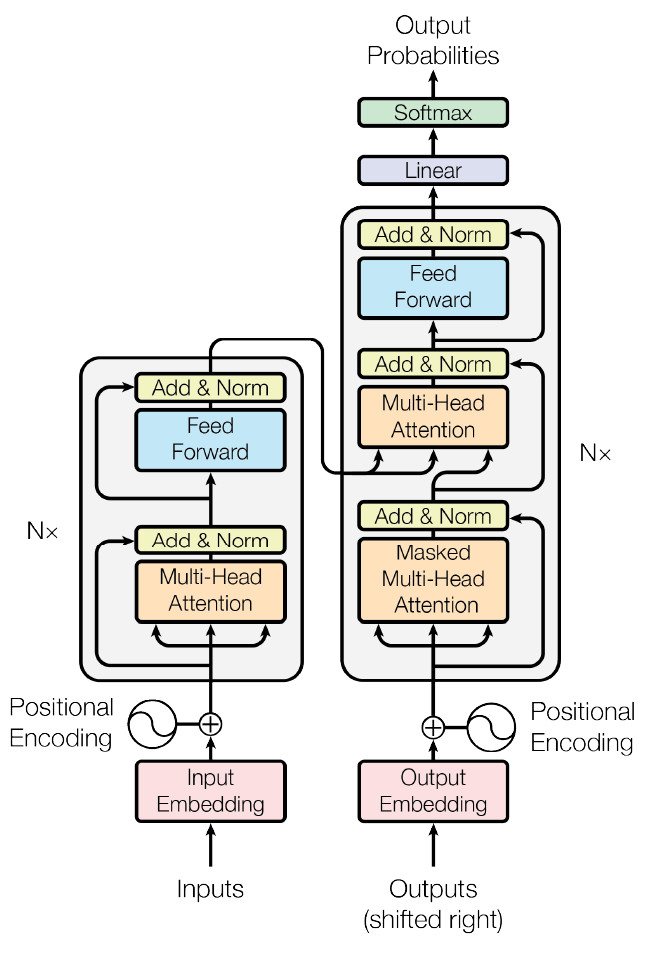
\includegraphics[width=0.8\columnwidth]{picture/Transfromer_architecture}
		%\captionsetup{font=scriptsize}
		\caption{
			\label{fig: Transformer} The Transformer - model architecture.
		}
	\end{figure}
	
	如Fig.\ref{fig: Transformer}所示,\textbf{Transformer}模型也是使用经典的encoer-decoder架构,由encoder和decoder两部分组成。
	
	上图的左半边用Nx框中,为encoder的一层。\textbf{encoder一共有6层这样的结构。}
	
	上图的右半边用Nx框中,为decoder的一层。\textbf{decoder一共有6层这样的结构。}
	
	输入序列经过\textbf{word embedding}和\textbf{positional encoding}相加后,输入到encoder。
	
	输出序列经过\textbf{word embedding}和\textbf{positional encoding}相加后,输入到decoder。
	
	最后,decoder输出的结果,经过一个线性层,然后计算softmax。
	
	\paragraph{Encoder}
	
	encoder由6层相同的层组成,每一层分别由两部分组成:
	
	\begin{itemize}
		\item {}
			第一部分是一个multi-head self-attention mechanism;
		\item {}
			第二部分是一个position-wise feed-forward network,是一个全连接层.
	\end{itemize}
	
	两个部分,都有一个\textbf{残差连接(residual connection)},然后接着一个\textbf{Layer Normalization}。
	
	
	\paragraph{Decoder}
	
	和encoder类似,decoder由6个相同的层组成,每一个层包括以下3个部分:
	
	\begin{itemize}
	\item {}
		第一个部分是multi-head self-attention mechanism
	\item {}
		第二部分是multi-head context-attention mechanism
	\item {}
		第三部分是一个position-wise feed-forward network
	\end{itemize}
	
	与encoder类似,上面三个部分的每一个部分,都有一个残差连接,后接一个Layer Normalization。
	
	但是,decoder出现了一个新的部分\textbf{multi-head context-attention}
	
	\subsubsection{Attention Mechanism}
	
	\textbf{Attention}是指,对于某个时刻的输出$y$,它在输入$x$上各个部分的注意力。这个注意力实际上可以理解为权重。
	
	\paragraph{Scaled dot-product attention}
	
	Transformer模型基于乘性注意力(multiplicative attention),采用\textbf{scaled dot-product attention},即\textbf{两个隐状态进行点积。}
	
	\begin{equation}
		\begin{aligned}
			\textbf{score}(\mathbf{s_t},\mathbf{h_i})=\frac{\mathbf{s_t^\top h_i}}{\sqrt{n}}
		\end{aligned}
		\label{eq: multiplicative attention}
	\end{equation}
	
	其中$h_i$为输入序列隐状态,$s_t$为输出序列的隐状态。
	
	\begin{figure}[htbp]
		% read manual to see what [ht] means and for other possible options
		\centering 
		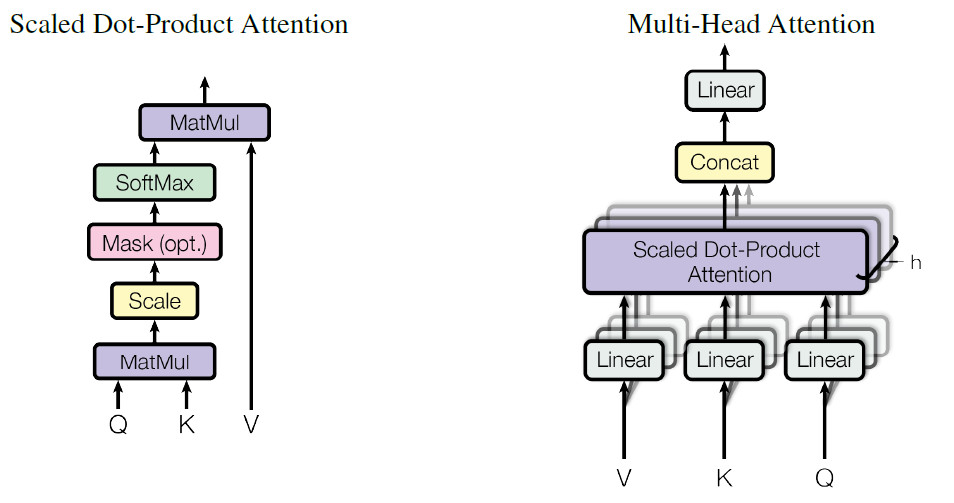
\includegraphics[width=0.8\columnwidth]{picture/Transfromer_attention}
		\captionsetup{font=scriptsize}
		\caption{
			\label{fig: Transformer_attention} (left) Scaled Dot-Product Attention. (right) Multi-Head Attention consists of several attention layers running in parallel.
		}
	\end{figure}
	
	\textbf{self-attention}实际上就是,\textbf{输出序列就是输入序列!}因此,计算自己的attention得分,就叫做self-attention!
	
	\textbf{context-attention}是encoder和decoder之间的attention。
	
	从Fig.\ref{fig: Transformer_attention}(left)看出,Transformer中的attention机制可以被描述为,通过确定$Q$和$K$之间的相似程度来选择$V$,
	\begin{equation}
		\begin{aligned}
			\textbf{Attention}(Q,K,V)=\text{softmax}(\frac{QK^\top}{\sqrt{d_k}})V
		\end{aligned}
		\label{eq: Transformer_attention}
	\end{equation}
	
	其中,$d_k$表示的是$K$的维度。\footnote{\textbf{为什么需要加上这个缩放因子$d_k$呢?}论文里给出了解释:对于$d_k$很大的时候,点积得到的结果维度很大,使得结果处于softmax函数梯度很小的区域。
		
	我们知道,梯度很小的情况,这对反向传播不利。为了克服这个负面影响,除以一个缩放因子,可以一定程度上减缓这种情况。}
	
	$K, Q, V$具体指代什么?
	\begin{itemize}
		\item {}
		
			在encoder的\textbf{self-attention}中,$Q, K, V$都来自同一个地方(相等),他们是上一层 encoder 的输出。对于第一层 encoder ,它们就是 word embedding 和 positional encoding 相加得到的输入。
		
		\item {}
		
			在decoder的self-attention中,$Q, K, V$都来自于同一个地方(相等),它们是上一层 decoder 的输出。对于第一层decoder,它们就是 word embedding 和 positional encoding 相加得到的输入。但是对于 decoder ,我们不希望它能获得下一个 time step (即将来的信息),因此我们需要进行 sequence masking 。

		\item {}
		
			在encoder-decoder attention中,$Q$来自于decoder的上一层的输出,$K$和$V$来自于encoder的输出,$K$和$V$是一样的。
			
		\item {}
			
			$Q$、$K$、$V$三者的维度一样,即 $d_q=d_k=d_v$。
	\end{itemize}
	
	\paragraph{Multi-head attention}
	
	什么是\textbf{multi-head attention}?
	
	如Fig.\ref{fig: Transformer_attention}(right)所示,作者发现将$Q,K,V$通过一个线性映射之后,分成 $h$ 份,对每一份进行 \textbf{scaled dot-product attention} 效果更好。然后,把各个部分的结果合并起来,再次经过线性映射,得到最终的输出。超参数 $h$ 表示的是 heads 数量\footnote{论文中的数量默认是8}。
	
	\begin{equation}
		\begin{aligned}
			& \textbf{MultiHead}(Q,K,V)=\textbf{Concat}(\textbf{head}_{1},\ldots,\textbf{head}_{h})W^{O}, \\
			& \textbf{head}_{i} = \textbf{Attention}(QW_i^Q,KW_i^K,VW_i^V)
		\end{aligned}
		\label{eq: Multi-head attention}
	\end{equation}
	
	\subsubsection{Layer normalization}
	
	\begin{itemize}
		\item {} Normalization 有很多种,但是它们都有一个共同的目的,那就是把输入转化成均值为 0 方差为 1 的数据。
		
		\item {} Normalization 是一种用于标准化数据的预处理技术\footnote{例如,假设我们有汽车租赁服务。首先,我们希望根据竞争对手的数据预测每辆车的合理价格。每辆车有两个特征:车龄和总行驶公里数。它们的范围可能非常不同,从 0 到 30 年不等,而距离可能从 0 到数十万公里。我们不希望特征在范围上存在这些差异,因为具有较高范围的值可能会使我们的模型产生偏差,从而赋予它们夸大的重要性。
		
		有两种主要方法可以标准化数据。最直接的方法是将其缩放到 0 到 1 的范围:
		
		\begin{equation}
			\begin{aligned}
				x_{normalized} = \frac{x-m}{x_{max}-x_{min}}
			\end{aligned}
			\label{eq: normalized_1}
		\end{equation}
		
		$x$是要标准化的数据点、$m$是数据集的平均值、$x_{max}$是最高值、$x_{min}$是最小值。该技术通常用于数据的输入。大范围的非标准化数据点可能会导致神经网络不稳定。相对较大的输入可能会级联到各层,从而导致梯度爆炸等问题。
		
		用于标准化数据的另一种技术是使用以下公式强制数据点的平均值为 0,标准差为 1:
		
		\begin{equation}
			\begin{aligned}
				x_{normalized} = \frac{x-m}{s}
			\end{aligned}
			\label{eq: normalized_2}
		\end{equation}
		
		$x$ 是要标准化的数据点、$m$是数据集的平均值、$s$是数据集的标准差。经过Eq.\ref{eq: normalized_2}后,每个数据点都模仿标准正态分布。拥有正态分布的所有特征,它们不会有偏差,因此,我们的模型会学得更好。
		}。换句话说,在同一范围内具有不同的数据源。在训练之前不对数据进行标准化可能会导致我们的网络出现问题,从而使训练变得更加困难并降低其学习速度。
	\end{itemize}
	
	
	\paragraph{Batch normalization}
	
	Batch normalization是在神经网络层之间而非在原始数据中完成的标准化方法,其主要思想是:\textbf{在每一层的每一批数据上进行归一化。}它是按照小批量而不是完整数据集完成的。它可以加快训练速度并使用更高的学习率,使学习变得容易。
	
	可以将Batch normalization的归一化公式定义为: 
	
	\begin{equation}
		\begin{aligned}
			z^{N} = \left( \frac{z-m_{z}}{s_{z}} \right)
		\end{aligned}
		\label{eq: Batch normalization}
	\end{equation}
	其中$m_z$是神经元输出的平均值和$s_z$神经元输出的标准差。
	
	我们可能会对输入数据进行归一化,但是经过该网络层的作用后,我们的的数据已经不再是归一化的了。随着这种情况的发展,数据的偏差越来越大,我的反向传播需要考虑到这些大的偏差,这就迫使我们只能使用较小的学习率来防止梯度消失或者梯度爆炸。
	
	
	Batch normalization的具体做法就是对每一小批数据,在批这个方向上做归一化。如下图所示:
	
	具体Batch normalization是如何应用的?
	
	\begin{figure}[htbp]
		\centering 
		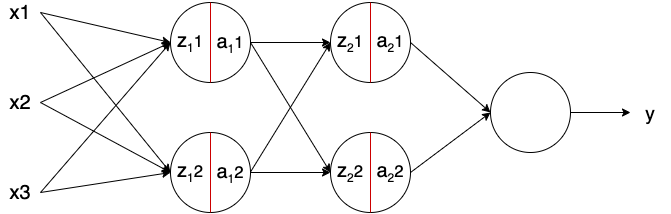
\includegraphics[width=0.8\columnwidth]{picture/neural-network}
		\captionsetup{font=scriptsize}
		\caption{
			\label{fig: Neural Network} 
			A conventional feedforward neural network.
		}
	\end{figure}
	
	在Fig.\ref{fig: Neural Network}中展示了一个常规的前馈神经网络,其中$x_i$是输入、$z$是神经元的输出、$a$是激活函数的输出、$y$是整个网络的输出。
	
	Batch normalization的好处是:
	
	\begin{itemize}
		\item {}
		
		\textbf{深度神经网络可以训练得更快:}虽然由于前向传播过程中的额外归一化计算和反向传播过程中需要训练的额外超参数,每次训练迭代都会变慢,但它应该收敛得更快;因此,训练总体上应该更快。	
		
		\item {}
		\textbf{更高的学习率:}梯度下降通常需要较小的学习率才能使网络收敛。随着网络变得更深,梯度在反向传播过程中变得更小,因此需要更多的迭代。使用批量归一化可以提高学习率,从而提高训练速度。
		
		\item {}
		\textbf{更容易初始化权重:}权重初始化可能很困难,特别是在创建更深的网络时。批量归一化降低了对初始起始重量的敏感性。
		
	\end{itemize}
	
	
	\section{Paper reading}
	
	\subsection{Ultra-High-Definition Low-Light Image Enhancement}
	
	\subsubsection{Introduce}
	
	设备捕捉超高清(UHD)图像和视频的能力对图像处理管道提出了新的要求。
	
	本文考虑了低光亮图像增强(LLIE)的任务,构建了两种不同分辨率的数据集Ultra High Definition Low-Light Image Enhancement(UHD-LOL),并在不同方法进行基准测试。作者提出一种基于\textbf{Transformer}的微光增强方法LLFormer。LLFormer的核心组件是基于轴的多头自注意和跨层注意融合块,显著降低了线性复杂度。
	
	\begin{figure}[htbp]
		% read manual to see what [ht] means and for other possible options
		\centering 
		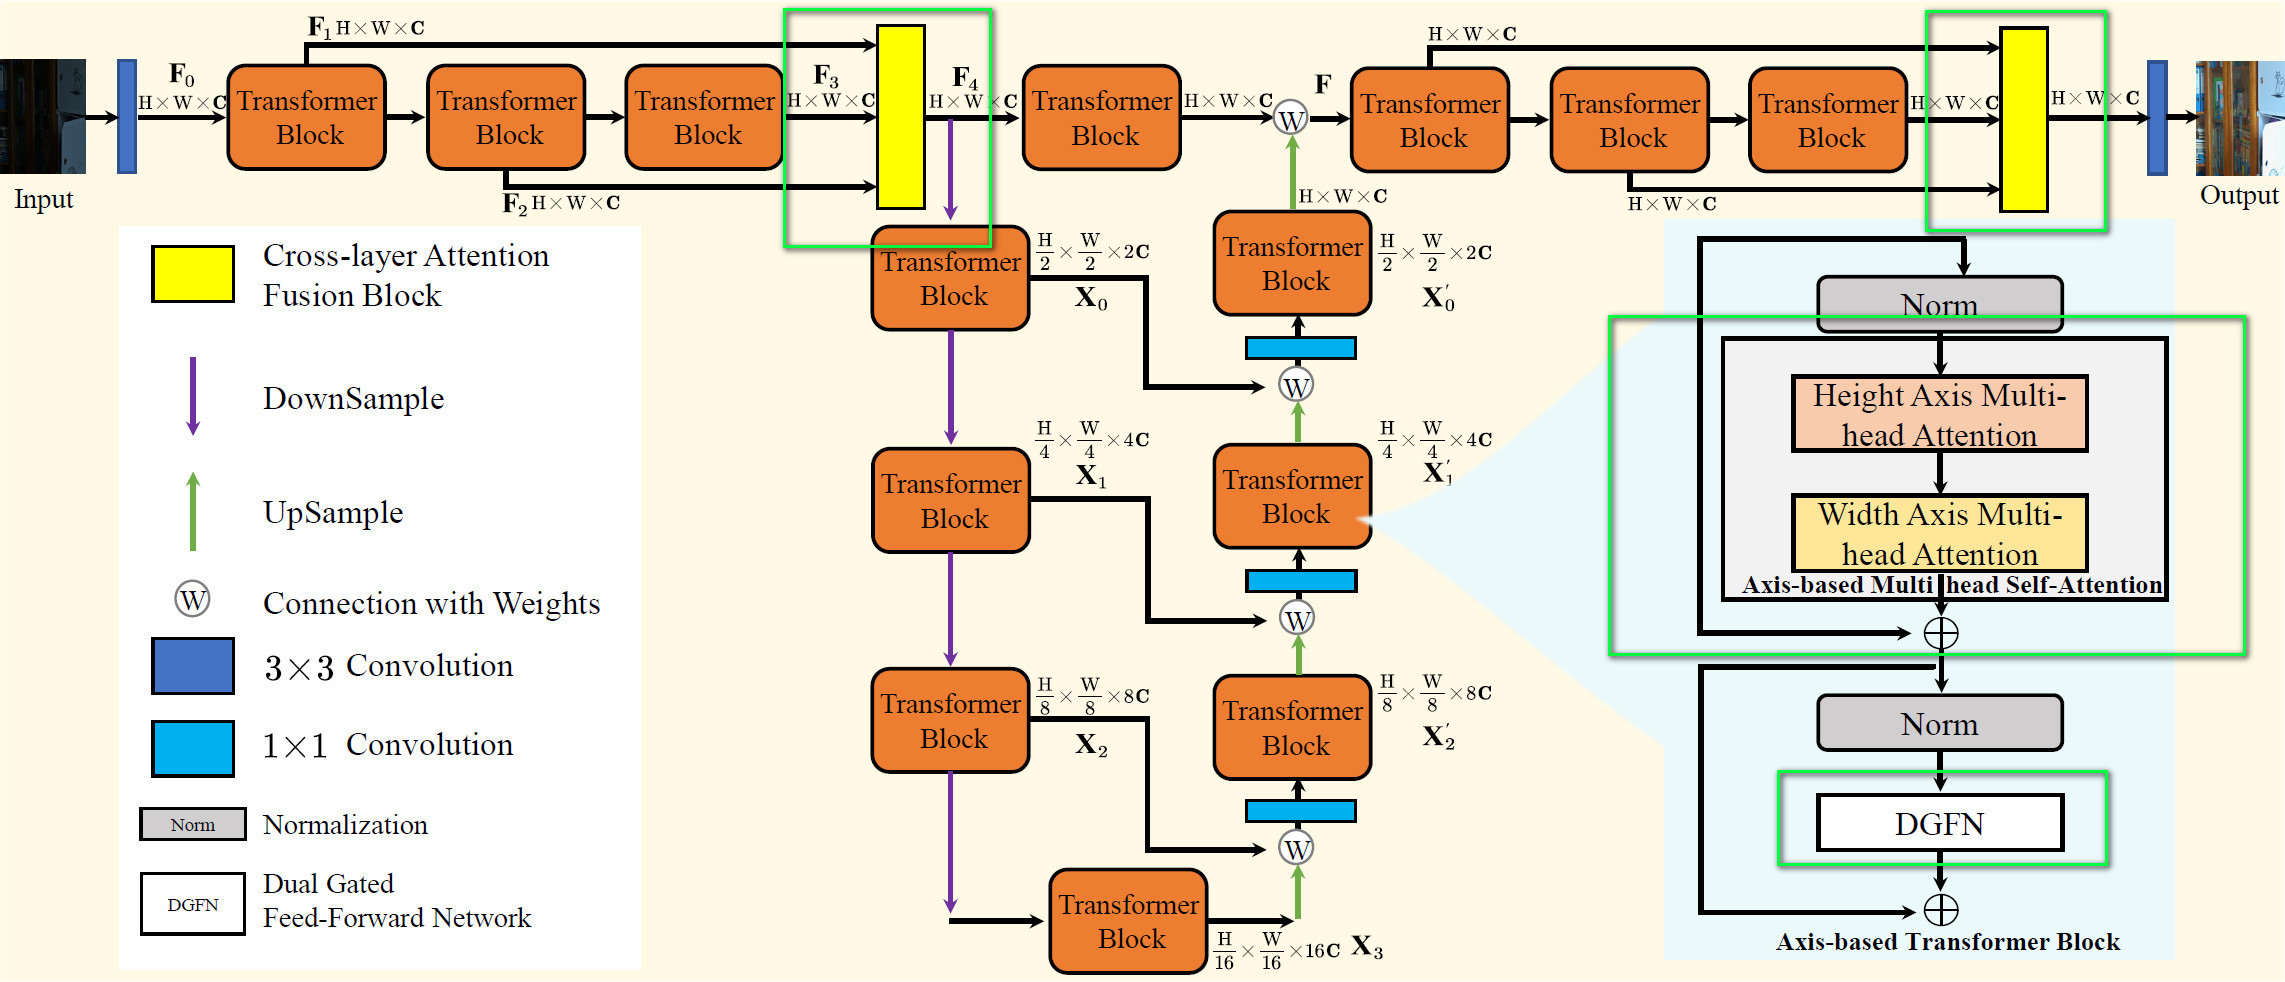
\includegraphics[width=\columnwidth]{picture/LLFormer_architecture}
		\captionsetup{font=scriptsize}
		\caption{
			\label{fig: LLFormer architecture} % spaces are big no-no withing labels
			% things like fig: are optional in the label but it helps
			% to orient yourself when you have multiple figures,
			% equations and tables
			\textbf{LLFormer architecture}. The core design of LLFormer includes an \colorbox{yellow}{axis-based transformer block} and a \colorbox{yellow}{cross-layer attention fusion block}. In the former, \colorbox{yellow}{axis-based multi-head self-attention} performs self-attention on the height and width axis across the channel dimension sequentially to reduce the computational complexity, and a \colorbox{yellow}{dual gated feed-forward network} employs a gated mechanism to focus more on useful features. The cross-layer attention fusion block learns the attention weights of features in different layers when fusing them.
			}
	\end{figure}
	LLFormer的核心设计包括一个基于轴的变压器块(Axis-based Transformer Block)和一个跨层注意力融合块(Dual Gated Feed-forward Network)。在前者中,基于轴的多头自注意在通道维度上依次对高度和宽度轴进行自注意,以降低计算复杂度,而双门控前馈网络采用门控机制来更多地关注有用的特征。跨层注意力融合块在融合不同层中的特征时学习它们的注意力权重。
	
	\subsubsection{Innovation}
	
	LLFormer 的整体框架如Fig.\ref{fig: LLFormer architecture}所示,可以看出和 Restormer 有些类似。作者改进了三个点:
	\begin{itemize}
		\item {(1)} Transformer block里面修改了attention;
		\item {(2)} Transformer block里修改了FFN;
		\item {(3)} 添加了cross-layer attention。
	\end{itemize}
	
	\paragraph{Axis-based Transformer Block}
	
	\textbf{Transformer}在图像修复中应用的难点在于计算复杂度高,在$Q$和$K$计算相似性时,对于输入为$(C,H,W)$的特征需要进行$(C,H,W) \times (C,H,W)$的矩阵运算。论文使用基于轴的多头注意力,因此,作者分为两个步骤,第一步相似性计算的是$H \times H$,叫做 \texttt{height-axis attention} 。第二步相似性计算的是 $W \times W$,叫做 \texttt{width-axis attention} 。(这里可以对比 Restormer,只是在C这个维度计算相似性)。。
	
	\paragraph{Dual Gated Feed-forward Network(DGFN)}
	
	在Restormer中,FFN有两个分支,其中有一个分支上使用GELU激活对另一个分支添加门控。
	在该文中,如图Fig.\ref{fig: Axis-based Transformer Block & Dual Gated Feed-forward Network(GDFN)}c,作者在FFN中引入双门控机制,提出双门控前馈网络 DGFN 来捕获特征中的更重要的信息。FFN两个分支都使用 GELU 激活,再互相给另外一个分支添加门控增强非线性建模能力。
	
	\begin{figure}[htbp]
		% read manual to see what [ht] means and for other possible options
		\centering 
		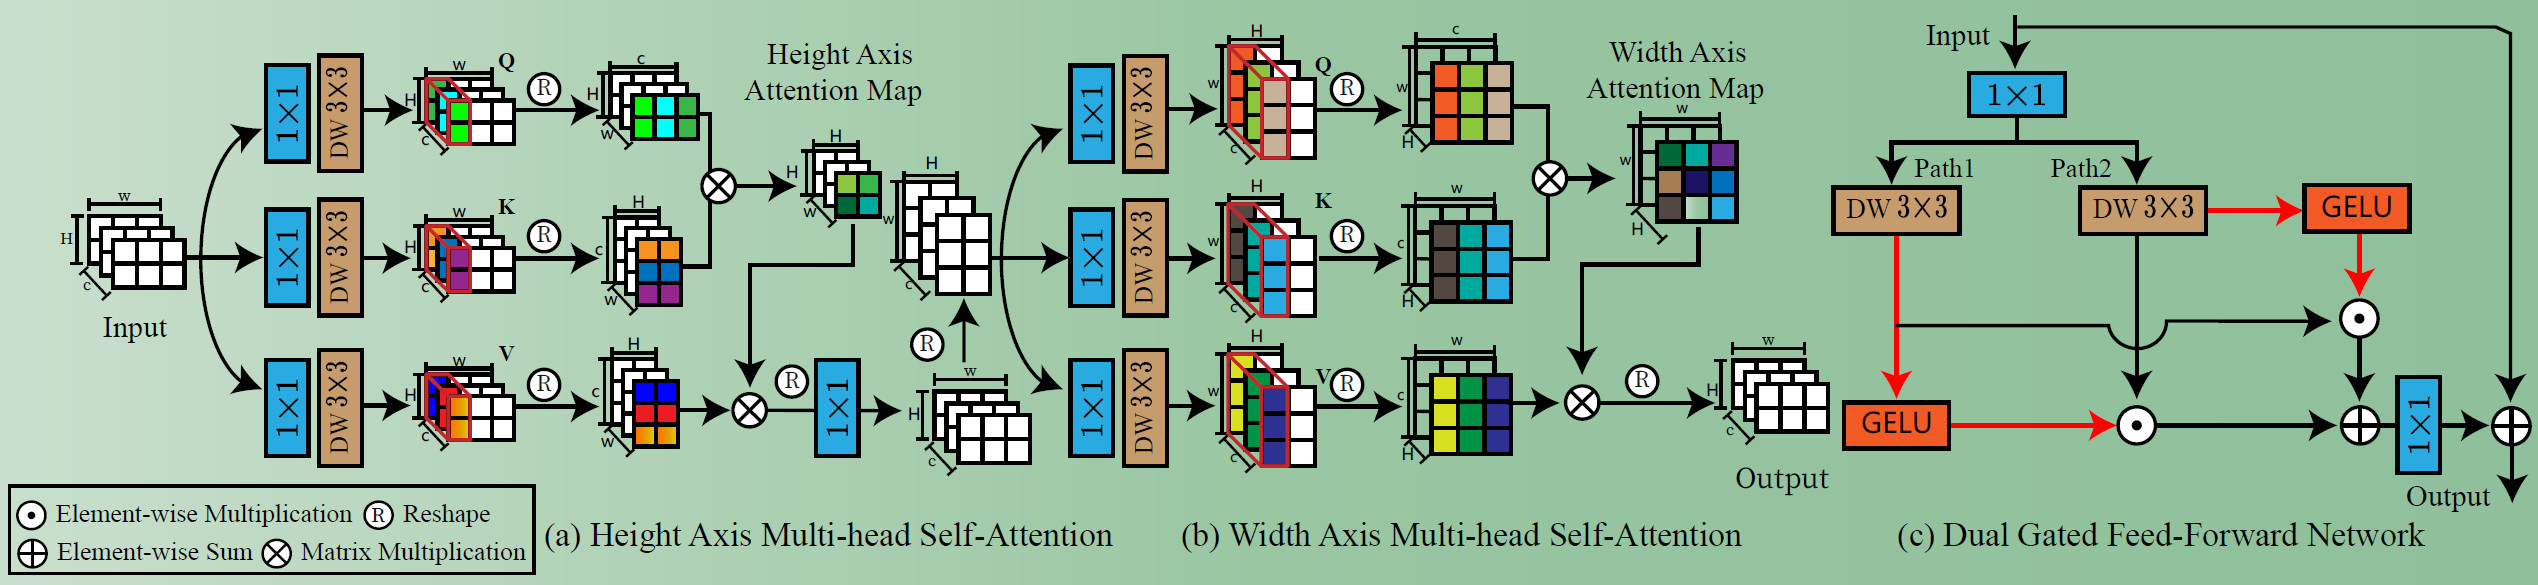
\includegraphics[width=\columnwidth]{picture/Axis_based_Transformer_Block_&_Dual_Gated_Feed-forward_Network(GDFN)}
		\captionsetup{font=scriptsize}
		\caption{
			\label{fig: Axis-based Transformer Block & Dual Gated Feed-forward Network(GDFN)} % spaces are big no-no withing labels
			% things like fig: are optional in the label but it helps
			% to orient yourself when you have multiple figures,
			% equations and tables
			The architecture of our Axis-based Multi-head Self-Attention and Dual Gated Feed-Forward Network. From left to right, the components are Height Axis Multi-head Attention, Width Axis Multi-head Attention, and Dual Gated Feed-Forward Network.
		}
	\end{figure}
	
	\begin{equation}
		\begin{aligned}
			& \mathbf{F}_\prime = \text{A-MSA} \left(\text{LN}(\textbf{F}_\textbf{in})\right) + \mathbf{F}_\mathbf{in}, \\
			& \mathbf{F}_\mathbf{out} = \text{DGFN} \left(\text{LN}\mathbf{F}^\prime)\right) + \mathbf{F}^\prime,
		\end{aligned}
		\label{eq: FFN}
	\end{equation}
	
	其中,\text{DGFN}公式如下:
	
	\begin{equation}
		\begin{aligned}
			& \mathbf{DG} = \phi \left(W_{3\times 3}^1 W_{1\times1}^1 \mathbf{Y} \right) \odot \left(W_{3\times3}^2 W_{1\times1}^2\mathbf{Y} \right)\\ 
			& \quad \quad  + \left(W_{3\times3}^1W_{1\times1}^1\mathbf{Y}\right) \odot \phi \left(W_{3\times3}^2 W_{1\times1}^2 \mathbf{Y}\right), \\
			& \hat{\mathbf{Y}} = W_{1\times1}\textbf{DG}\left(\mathbf{Y}\right) + \mathbf{Y}
		\end{aligned}
		\label{eq: DGFN}
	\end{equation}
	
	\paragraph{Cross-layer Attention Fusion Block}
	
	\begin{figure}[htbp]
		% read manual to see what [ht] means and for other possible options
		\centering 
		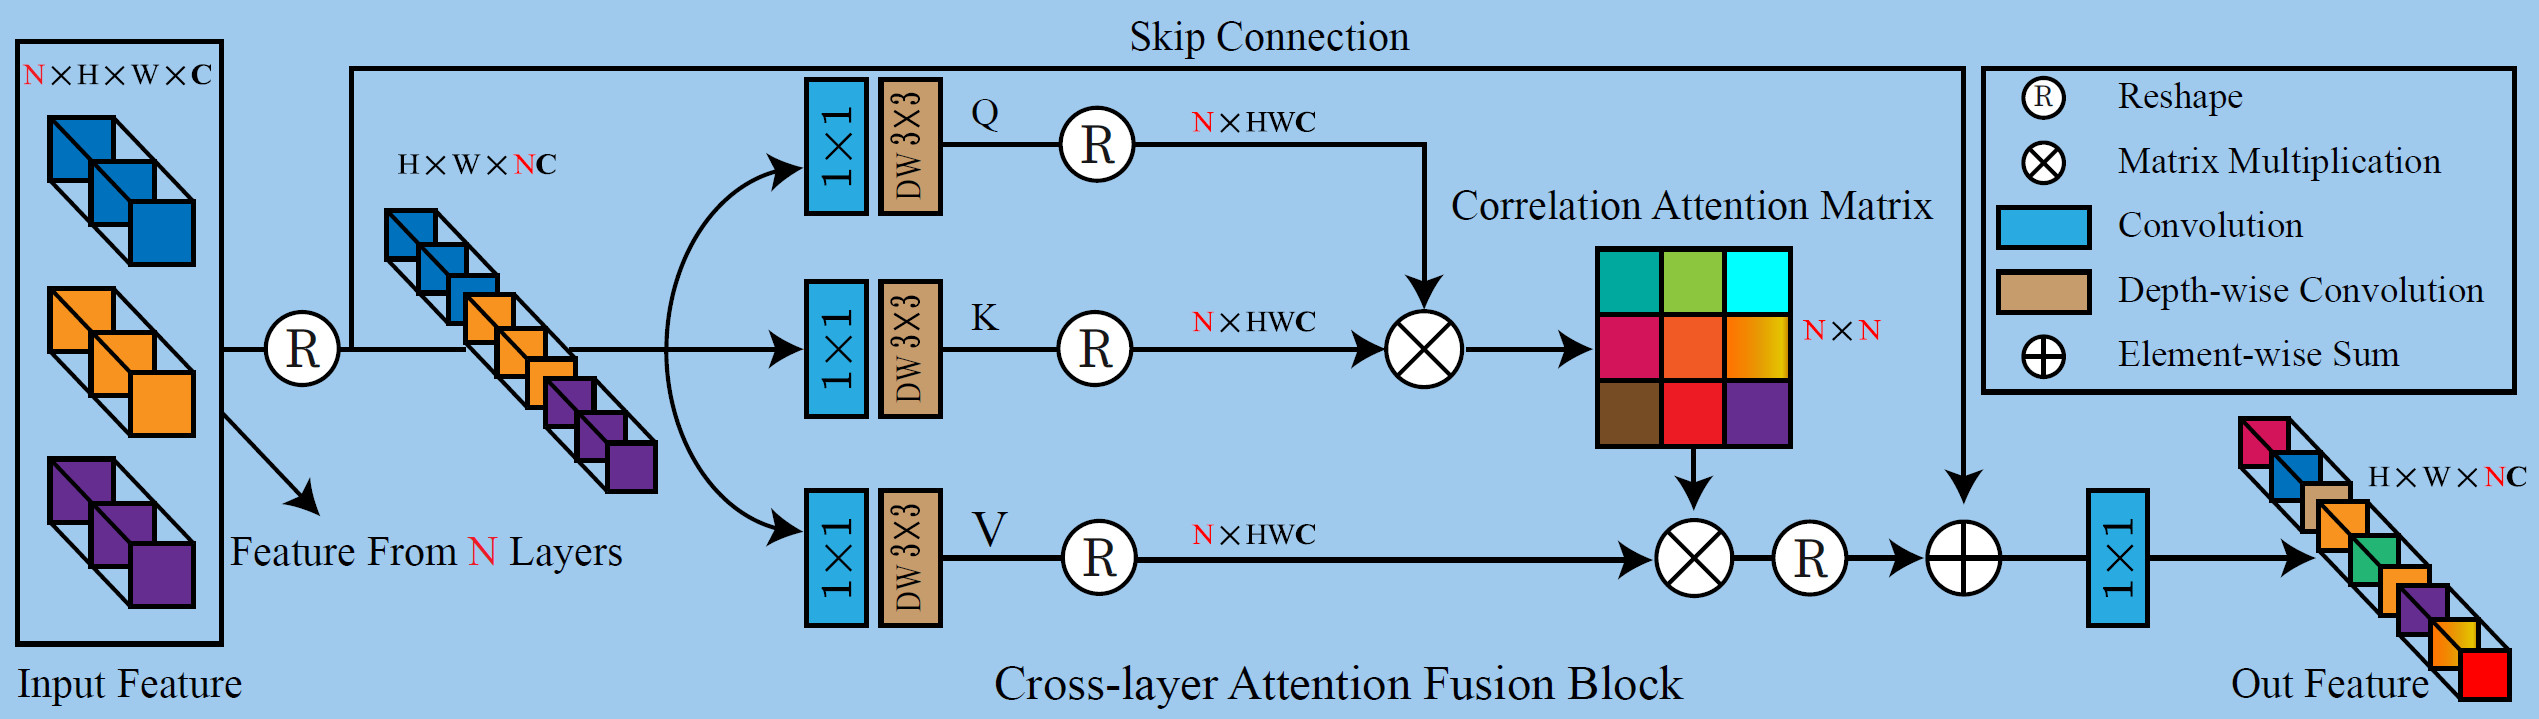
\includegraphics[width=\columnwidth]{picture/Cross-layer_Attention_Fusion_Block}
		\captionsetup{font=scriptsize}
		\caption{
			\label{fig: Cross-layer_Attention_Fusion_Block} % spaces are big no-no withing labels
			% things like fig: are optional in the label but it helps
			% to orient yourself when you have multiple figures,
			% equations and tables
			The architecture of the proposed Cross-layer Attention Fusion Block. This block efficiently integrates features from different layers with a layer correlation attention matrix.
		}
	\end{figure}
	
	 网络一般有多层,但大多方法没有考虑层与层之间特征的关联,限制了表示能力。论文使用cross-layer attention获取不同层特征间的相关性并融合。从论文整体架构图中可看到,网络输入有三个Transformer block,能得到三个特征输出。论文通过cross-layer attention 运算,计算一个3x3的相似性矩阵,给输入的特征进行加权,从而达到强调重要特征、抑制不重要特征的作用。(不同层的激活是对特定类别的响应,并且可以使用子注意力机制自适应地学习特征相关性。)
	
	\begin{equation}
		\begin{aligned}
			& \hat{\mathbf{F}}_{\mathbf{out}} = W_{1\times1}^1 \text{Layer\_Attention}(\hat{\mathbf{Q}}, \hat{\mathbf{K}}, \hat{\mathbf{V}}) + \hat{\mathbf{F}_{\mathbf{in}}},\\ 
			& \text{Layer\_Attention}(\hat{\mathbf{Q}}, \hat{\mathbf{K}}, \hat{\mathbf{V}}) = \hat{\mathbf{V}}\text{softmax}\left(\hat{\mathbf{Q}}\hat{\mathbf{K}}/\mathbf{\alpha}\right), 
		\end{aligned}
		\label{eq: DGFN}
	\end{equation}
	
	\subsubsection{Result}
	
	结果见Fig.\ref{fig: result_in_UHD-LOL} 和 Fig.\ref{fig: result_in_LOL_and_MIT}
	
	\begin{figure}[htbp]
		% read manual to see what [ht] means and for other possible options
		\centering 
		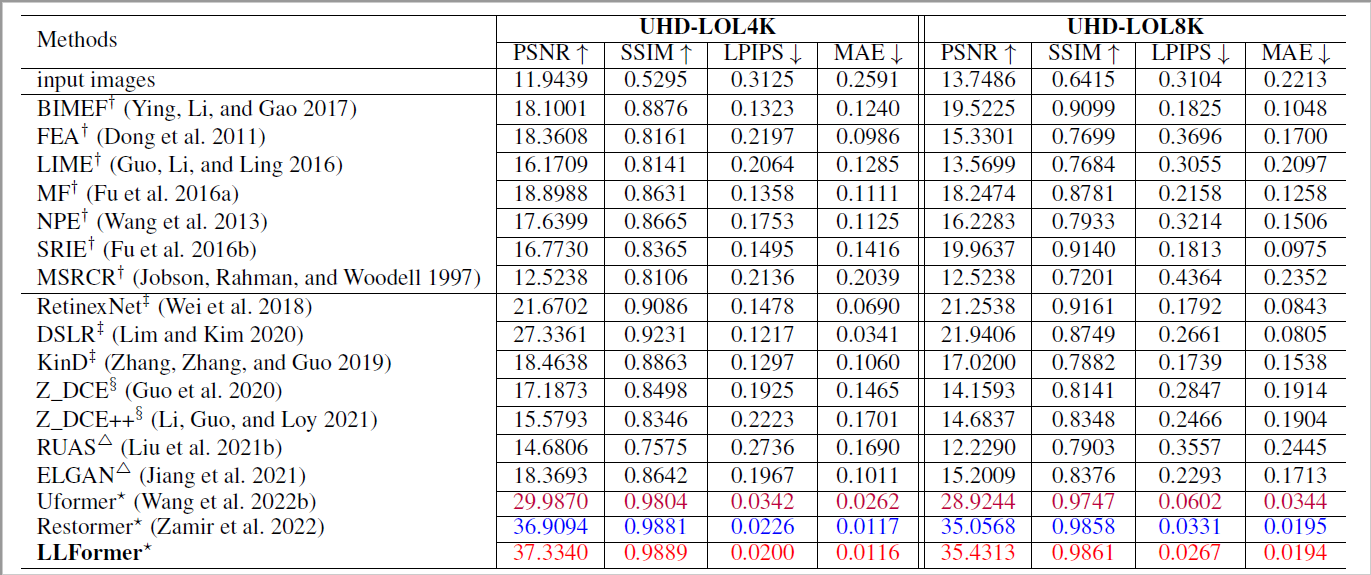
\includegraphics[width=\columnwidth]{picture/Results_on_UHD-LOL}
		\captionsetup{font=scriptsize}
		\caption{
			\label{fig: result_in_UHD-LOL} % spaces are big no-no withing labels
			% things like fig: are optional in the label but it helps
			% to orient yourself when you have multiple figures,
			% equations and tables
			Benchmarking study on the UHD-LOL4K and UHD-LOL8K subsets. $\dag$; $\ddag$; $\S$;$\triangle$ and ? indicate the traditional methods, supervised CNN-based methods, unsupervised CNN-based methods, zero-shot methods and transformer-based methods. The top three results are marked in red, blue and purple, respectively.
			Input
		}
	\end{figure}
	
	\begin{figure}[htbp]
		% read manual to see what [ht] means and for other possible options
		\centering 
		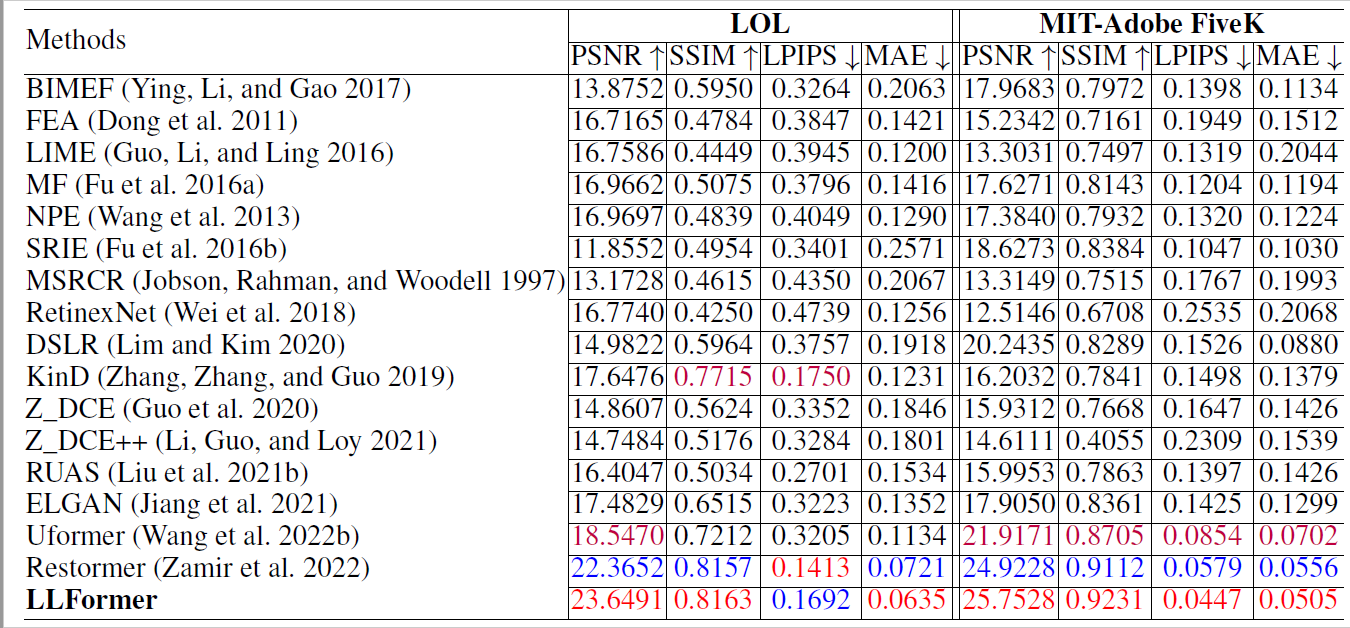
\includegraphics[width=\columnwidth]{picture/Results_on_LOL_and_MIT-Adobe_FiveK}
		\captionsetup{font=scriptsize}
		\caption{
			\label{fig: result_in_LOL_and_MIT} % spaces are big no-no withing labels
			% things like fig: are optional in the label but it helps
			% to orient yourself when you have multiple figures,
			% equations and tables
			Comparison results on LOL and MIT-Adobe FiveK datasets in terms of PSNR, SSIM, LPIPS and MAE. The top three results are marked in red, blue and purple, respectively. Same as (Zamir et al. 2020), we consider images from expert C for the MIT-Adobe FiveK dataset.
		}
	\end{figure}
	
	\section{个人工作进展}
	
	\subsection{思考}
	
	\begin{itemize}
		\item [(1)] 以后的工作中如果有涉及可以尝试使用双门控来增强局部信息的提取能力,在有依据的情况下可以将注意力计算分解为多步,通过多步计算来控制计算量。
		
		\item [(2)] Self-attention Module 到底在 CV 能做什么?
		
	\end{itemize}

	
	\section{下周工作计划}
	
	(1) 继续了解Transformer结构原理,去了解Mask和Positional Encoding的部分。
	
	(2) 了解的Transformer模型是通用模型,而且应用在NLP领域,具体细化到CV领域,会有领域差异,目前已经了解到的应用到CV领域的Transformer模型,有ViT,DeiT,Swin,对它们进行一个初步的了解
	
	%	\section{Analysis}
	
	%	In this section you will need to show your experimental results. Use tables and
	%	graphs when it is possible. Table~\ref{tbl:bins} is an example.
	
	%	\begin{table}[ht]
		%		\begin{center}
			%			\caption{Every table needs a caption.}
			%			\label{tbl:bins} % spaces are big no-no withing labels
			%			\begin{tabular}{|ccc|} 
				%				\hline
				%				\multicolumn{1}{|c}{$x$ (m)} & \multicolumn{1}{c|}{$V$ (V)} & \multicolumn{1}{c|}{$V$ (V)} \\
				%				\hline
				%				0.0044151 &   0.0030871 &   0.0030871\\
				%				0.0021633 &   0.0021343 &   0.0030871\\
				%				0.0003600 &   0.0018642 &   0.0030871\\
				%				0.0023831 &   0.0013287 &   0.0030871\\
				%				\hline
				%			\end{tabular}
			%		\end{center}
		%	\end{table}
	%	
	%	Analysis of equation~\ref{eq:aperp} shows ...
	%	
	%	Note: this section can be integrated with the previous one as long as you
	%	address the issue. Here explain how you determine uncertainties for different
	%	measured values. Suppose that in the experiment you make a series of
	%	measurements of a resistance of the wire $R$ for different applied voltages
	%	$V$, then you calculate the temperature from the resistance using a known
	%	equation and make a plot  temperature vs. voltage squared. Again suppose that
	%	this dependence is expected to be linear~\cite{Cyr}, and the proportionality coefficient
	%	is extracted from the graph. Then what you need to explain is that for the
	%	resistance and the voltage the uncertainties are instrumental (since each
	%	measurements in done only once), and they are $\dots$. Then give an equation
	%	for calculating the uncertainty of the temperature from the resistance
	%	uncertainty. Finally explain how the uncertainty of the slop of the graph was
	%	found (computer fitting, graphical method, \emph{etc}.)
	%	
	%	If in the process of data analysis you found any noticeable systematic
	%	error(s), you have to explain them in this section of the report.
	%	
	%	It is also recommended to plot the data graphically to efficiently illustrate
	%	any points of discussion. For example, it is easy to conclude that the
	%	experiment and theory match each other rather well if you look at
	%	Fig.~\ref{fig:samplesetup} and Fig.~\ref{fig:exp_plots}.
	%	
	%	\begin{figure}[ht] 
		%		\centering
		%		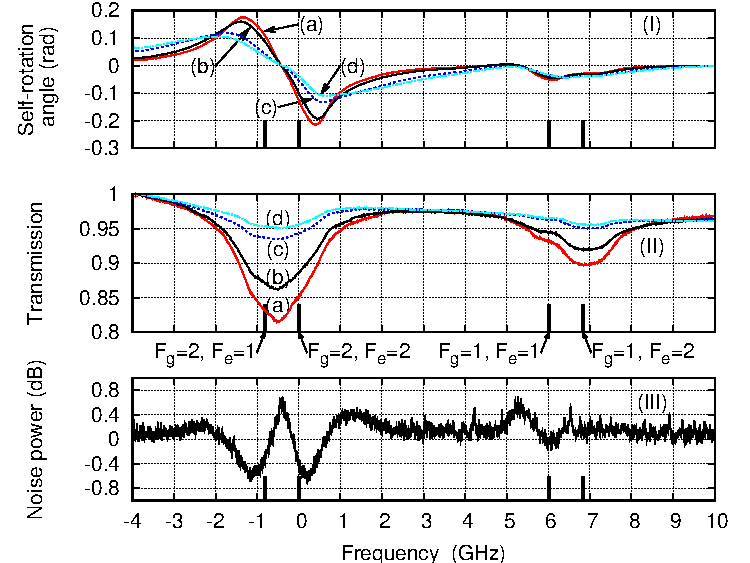
\includegraphics[width=0.5\columnwidth]{sr_squeezing_vs_detuning}
		%		
		%		% some figures do not need to be too wide
		%		\caption{
			%			\label{fig:exp_plots}  
			%			Every plot must have axes labeled.
			%		}
		%	\end{figure}
	
	
	%	\section{Conclusions}
	%	Here you briefly summarize your findings.
	
	%++++++++++++++++++++++++++++++++++++++++
	% References section will be created automatically 
	% with inclusion of "thebibliography" environment
	% as it shown below. See text starting with line
	% \begin{thebibliography}{99}
		% Note: with this approach it is YOUR responsibility to put them in order
		% of appearance.
		
		\renewcommand{\refname}{References}
		
		
		%	\begin{thebibliography}{00}
			
			%		\bibitem{b1}\label{cite:b1}
			%		W. Wang, C. Wei, W. Yang and J. Liu, "GLADNet: Low-Light Enhancement Network with Global Awareness," 2018 13th IEEE International Conference on Automatic Face \& Gesture Recognition (FG 2018), Xi'an, China, 2018, pp. 751-755, DOI: 10.1109/FG.2018.00118.
			
			%		\bibitem{b2}\label{cite:b2}
			%		A.\ Mahajan, K.\ Somaraj and M. Sameer, "Adopting Artificial Intelligence Powered ConvNet To Detect Epileptic Seizures," 2020 IEEE-EMBS Conference on Biomedical Engineering and Sciences (IECBES), Langkawi Island, Malaysia, 2021, pp. 427-432, DOI: 10.1109/IECBES48179.2021.9398832.
			
			%		\bibitem{Cyr}
			%		N.\ Cyr, M.\ T$\hat{e}$tu, and M.\ Breton,
			% "All-optical microwave frequency standard: a proposal,"
			%		IEEE Trans.\ Instrum.\ Meas.\ \textbf{42}, 640 (1993).
			
			
			
			%	\end{thebibliography}
		
		\bibliographystyle{unsrt}
		\bibliography{reference}
		
		
	\end{document}
